\documentclass[journal,12pt,onecolumn]{IEEEtran}
\usepackage{cite}
\usepackage{graphicx}
\usepackage{amsmath,amssymb,amsfonts,amsthm}
\usepackage{algorithmic}
\usepackage{graphicx}
\usepackage{textcomp}
\usepackage{xcolor}
\usepackage{txfonts}
\usepackage{listings}
\usepackage{enumitem}
\usepackage{mathtools}
\usepackage{gensymb}
\usepackage{comment}
\usepackage[breaklinks=true]{hyperref}
\usepackage{tkz-euclide} 
\usepackage{listings}
\usepackage{gvv}                                        
%\def\inputGnumericTable{}                                 
\usepackage[latin1]{inputenc}
\usetikzlibrary{arrows.meta, positioning}
\usepackage{xparse}
\usepackage{color}                                            
\usepackage{array}                                            
\usepackage{longtable}                                       
\usepackage{calc}                                             
\usepackage{multirow}
\usepackage{multicol}
\usepackage{hhline}                                           
\usepackage{ifthen}                                           
\usepackage{lscape}
\usepackage{tabularx}
\usepackage{array}
\usepackage{float}
\newtheorem{theorem}{Theorem}[section]
\newtheorem{problem}{Problem}
\newtheorem{proposition}{Proposition}[section]
\newtheorem{lemma}{Lemma}[section]
\newtheorem{corollary}[theorem]{Corollary}
\newtheorem{example}{Example}[section]
\newtheorem{definition}[problem]{Definition}
\newcommand{\BEQA}{\begin{eqnarray}}
\newcommand{\EEQA}{\end{eqnarray}}
\usepackage{float}
%\newcommand{\define}{\stackrel{\triangle}{=}}
\theoremstyle{remark}
\usepackage{circuitikz}
\usepackage{tikz}
\usepackage{ragged2e}

\title{GATE Petroleum Engineering (PE) 2024}
\author{Organizing Institute: IISc Bengaluru}
\date{}

\begin{document}

\maketitle

\section*{General Aptitude (GA)}

\subsection*{Questions 1 to 5 Carry ONE Mark Each}
\begin{enumerate}
\item If '---' denotes increasing order of intensity, then the meaning of the words [drizzle $\rightarrow$ rain $\rightarrow$ downpour] is analogous to [\underline{\hspace{1.5cm}} $\rightarrow$ quarrel $\rightarrow$ feud]. Which one of the given options is appropriate to fill the blank?
\begin{enumerate}
\begin{multicols}{2}
    \item bicker
    \item bog
    \item dither
    \item dodge
\end{multicols}
\end{enumerate}
\hfill{\brak{\text{GATE PE 2024}}}


\item  Statements: 
\begin{enumerate}
    \item All heroes are winners.
    \item All winners are lucky people.
\end{enumerate}
Inferences:
\begin{enumerate}[label=(\Roman*)]
    \item All lucky people are heroes.
    \item Some lucky people are heroes.
    \item Some winners are heroes.
\end{enumerate}
Which of the above inferences can be logically deduced from statements 1 and 2?
\begin{enumerate}
\begin{multicols}{2}
    \item Only I and II
    \item Only II and III
    \item Only I and III
    \item Only III
   \end{multicols} 
\end{enumerate}
\hfill{\brak{\text{GATE PE 2024}}}



\item  A student was supposed to multiply a positive real number $p$ with another positive real number $q$. Instead, the student divided $p$ by $q$. If the percentage error in the student's answer is 80\%, the value of $q$ is
\begin{enumerate}
\begin{multicols}{2}
    \item 5
    \item $\sqrt{2}$
    \item 2
    \item $\sqrt{5}$
 \end{multicols}   
\end{enumerate}
\hfill{\brak{\text{GATE PE 2024}}}



 \item If the sum of the first 20 consecutive positive odd numbers is divided by $20^2$, the result is
\begin{enumerate}
\begin{multicols}{2}
    \item 1
    \item 20
    \item 2
    \item $\frac{1}{2}$
    \end{multicols}
\end{enumerate}
\hfill{\brak{\text{GATE PE 2024}}}



\item  The ratio of the number of girls to boys in class VIII is the same as the ratio of the number of boys to girls in class IX. The total number of students \brak{\text{boys and girls}} in classes VIII and IX is 450 and 360, respectively. If the number of girls in classes VIII and IX is the same, then the number of girls in each class is
\begin{enumerate}
\begin{multicols}{2}
    \item 150
    \item 200
    \item 250
    \item 175
  \end{multicols}  
\end{enumerate}
\hfill{\brak{\text{GATE PE 2024}}}
\item  In the given text, the blanks are numbered (i)$-$\brak{iv}. Select the best match for all the blanks. \\
Yoko Roi stands \underline{\brak{i}} as an author for standing \underline{\brak{ii}} as an honorary fellow, after she stood \underline{\brak{iii}} her writings that stand \underline{\brak{iv}} the freedom of speech.
\begin{enumerate}
\begin{multicols}{2}
    \item i out ii down iii in iv for
    \item i down ii out iii by iv in
    \item i down ii out iii for iv in
    \item i out ii down iii by iv for
    \end{multicols}
\end{enumerate}
\hfill{\brak{\text{GATE PE 2024}}}



 \item Seven identical cylindrical chalk-sticks are fitted tightly in a cylindrical container. The figure below shows the arrangement of the chalk-sticks inside the cylinder.
 \begin{figure}[h]
     \centering
     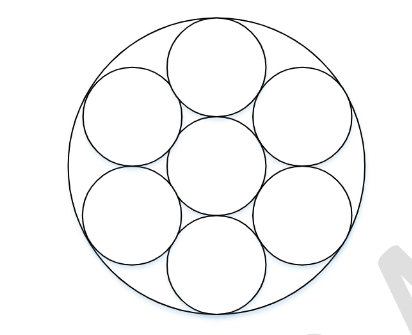
\includegraphics[width=0.5\columnwidth]{figs/im 1.jpeg}
     \caption{}
     \label{fig:placeholder}
 \end{figure}

The length of the container is equal to the length of the chalk-sticks. The ratio of the occupied space to the empty space of the container is
\begin{enumerate}
\begin{multicols}{2}
    \item $\frac{5}{2}$
    \item $\frac{7}{2}$
    \item $\frac{9}{2}$
    \item 3
    \end{multicols}
\end{enumerate}
\hfill{\brak{\text{GATE PE 2024}}}
 \item The plot below shows the relationship between the mortality risk of cardiovascular disease and the number of steps a person walks per day. Based on the data, which one of the following options is true?
\begin{figure}[h]
    \centering
    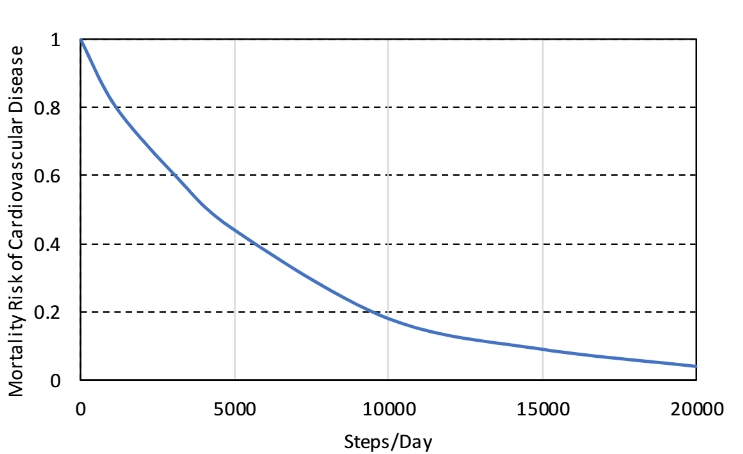
\includegraphics[width=0.5\columnwidth]{figs/im 2.jpeg}
    \caption{}
    \label{fig:placeholder}
\end{figure}


\begin{enumerate}
    \item The risk reduction on increasing the steps/day from 0 to 10000 is less than the risk reduction on increasing the steps/day from 10000 to 20000.
    \item The risk reduction on increasing the steps/day from 0 to 5000 is less than the risk reduction on increasing the steps/day from 15000 to 20000.
    \item For any 5000 increment in steps/day the largest risk reduction occurs on going from 0 to 5000.
    \item For any 5000 increment in steps/day the largest risk reduction occurs on going from 15000 to 20000.
\end{enumerate}
\hfill{\brak{\text{GATE PE 2024}}}



\item  Five cubes of identical size and another smaller cube are assembled as shown in Figure A. If viewed from direction $X$, the planar image of the assembly appears as Figure B.
\begin{figure}[h]
    \centering
    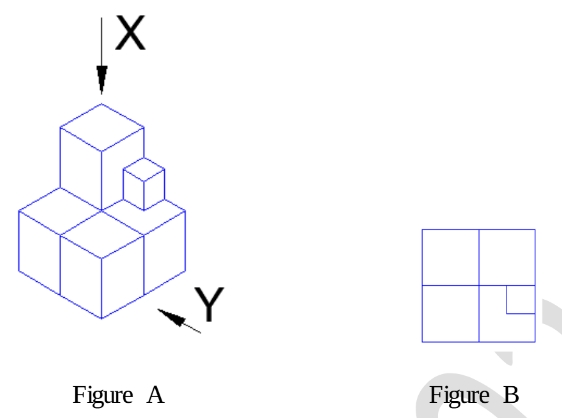
\includegraphics[width=0.5\columnwidth]{figs/im 3.jpeg}
    \caption{}
    \label{fig:placeholder}
\end{figure}\\
If viewed from direction $Y$, the planar image of the assembly (Figure A) will appear as
\begin{enumerate}
    \item  
\includegraphics[width=0.2\linewidth]{figs/im 4 1.jpeg}
        
    \item 
        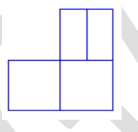
\includegraphics[width=0.2\linewidth]{figs/im 4 2.jpeg}
        
       
     \item 
        
\includegraphics[width=0.2\linewidth]{figs/im 4 3.jpeg}
       
     \item
        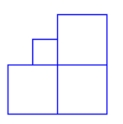
\includegraphics[width=0.2\linewidth]{figs/im 4 4.jpeg}
      
\end{enumerate}
\hfill{\brak{\text{GATE PE 2024}}}
\item  Visualize a cube that is held with one of the four body diagonals aligned to the vertical axis. Rotate the cube about this axis such that its view remains unchanged. The magnitude of the minimum angle of rotation is
\begin{enumerate}
\begin{multicols}{2}
    \item 120°
    \item 60°
    \item 90°
    \item 180°
    \end{multicols}
\end{enumerate}
\hfill{\brak{\text{GATE PE 2024}}}



\section*{Petroleum Engineering (PE)}



 \item A complex number is defined as $z = x + iy$ with $i = \sqrt{-1}$. $\bar{z}$ is the complex conjugate of $z$. The imaginary part of $(2z + 4\bar{z} + 4iy)$ is \underline{\hspace{1cm}}.
\begin{enumerate}
\begin{multicols}{2}
    \item 6
    \item 2
    \item 2$y$
    \item 3$y$
  \end{multicols}  
\end{enumerate}
\hfill{\brak{\text{GATE PE 2024}}}
 \item The solution of the initial value problem given by
 \begin{align}
 y'' + y' - 2y = 0\\ 
 y(0) = 3\\ 
 y'(0) = 6
 \end{align}

\begin{enumerate}
\begin{multicols}{2}
    \item $4e^x + e^{-2x}$
    \item $4e^x - e^{-2x}$
    \item $4e^x + 3e^{-2x}$
    \item $4e^{-2x} - 3e^x$
    \end{multicols}
\end{enumerate}
\hfill{\brak{\text{GATE PE 2024}}}



 \item open flow potential of a well is the
\begin{enumerate}
    \item maximum theoretical flow rate of reservoir fluid that a well can deliver
    \item minimum theoretical flow rate of reservoir fluid that a well can deliver
    \item flow rate of reservoir fluid from a well when the sandface pressure is 100 psia
    \item minimum flow rate of reservoir fluid when a well is stimulated
\end{enumerate}
\hfill{\brak{\text{GATE PE 2024}}}



\item  A constant composition expansion \brak{CCE} test is conducted on a slightly compressible reservoir fluid sample in a pressure-volume-temperature \brak{PVT} cell at 130°F. The data on the relative fluid volume $\left(\frac{V}{V_{\text{sat}}}\right)$ with pressure is given below:

\begin{table}[h]
\centering
\[
\begin{array}{|c|c|}
\hline
\textbf{Pressure (psia)} & \textbf{Relative fluid volume }\left(\tfrac{V}{V_{\text{sat}}}\right) \\
\hline
2530 & 0.967 \\
1650 & 0.987 \\
1425 & 0.992 \\
1250 & 1.000 \\
1128 & 1.021 \\
1095 & 1.038 \\
\hline
\end{array}
\]
\caption{Pressure vs. relative fluid volume}
\label{tab:fluid_volume}
\end{table}


The bubble point pressure \brak{psia} of the reservoir fluid is
\begin{enumerate}
\begin{multicols}{2}
    \item 2530
    \item 1650
    \item 1250
    \item 1095
   \end{multicols} 
\end{enumerate}
\hfill{\brak{\text{GATE PE 2024}}}



 \item Marsh funnel viscosity is reported as number of seconds required for one quart of drilling fluid sample to flow out of a Marsh funnel. The time of efflux of one quart of fresh water from a Marsh funnel at $70\pm5$ F is \underline{\hspace{1cm}} seconds.
\begin{enumerate}
\begin{multicols}{2}
    \item 21$\pm$0.5
    \item 26$\pm$0.5
    \item 31$\pm$0.5
    \item 36$\pm$0.5
    \end{multicols}
\end{enumerate}
\hfill{\brak{\text{GATE PE 2024}}}


\item  From the options given below, identify the process through which coal bed methane is produced.
\begin{enumerate}
    \item Underground coal gasification
    \item Open cast mining of coal
    \item Depressurization, using vertical/horizontal wells
    \item Underground coal combustion
\end{enumerate}
\hfill{\brak{\text{GATE PE 2024}}}



\item  Gas-liquid flow regimes for horizontal pipelines are shown below. Identify the correct pair from the list given below.
\begin{figure}[h]
    \centering
    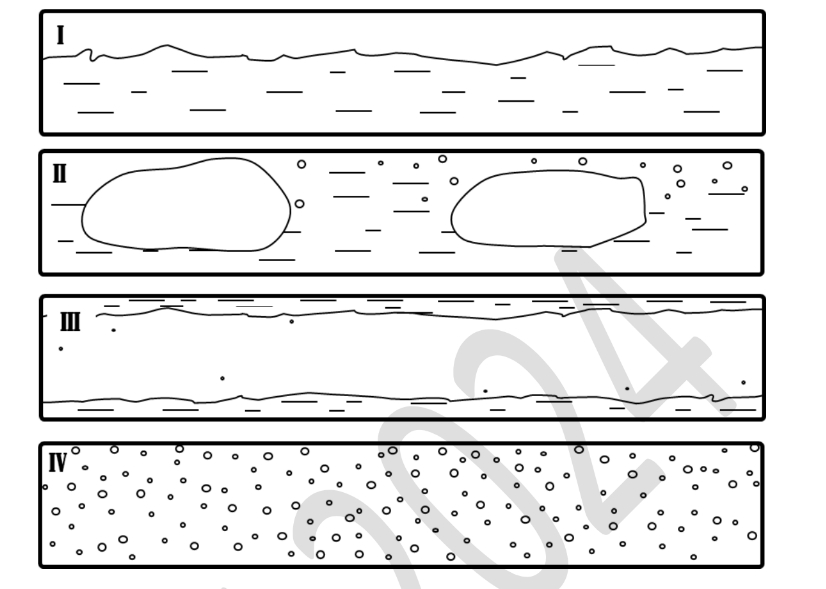
\includegraphics[width=0.5\columnwidth]{figs/im 5.jpeg}
    \caption{}
    \label{fig:placeholder}
\end{figure}
\begin{enumerate}
    \item I - Stratified; II - Slug; III - Annular; IV - Bubbly
    \item I - Slug; II - Bubbly; III - Annular; IV - Stratified
    \item I - Annular; II - Slug; III - Stratified; IV - Bubbly
    \item I - Slug; II - Stratified; III - Bubbly; IV - Annular
\end{enumerate}
\hfill{\brak{\text{GATE PE 2024}}}



\item  The speed of Tsunami is a function of
\begin{enumerate}
\begin{multicols}{2}
    \item only water depth
    \item only wave height
    \item both water depth and wave height
    \item both wind speed and wave height
    \end{multicols}
\end{enumerate}
\hfill{\brak{\text{GATE PE 2024}}}



\item  Which ONE of the following is a POSITIVELY BUOYANT floating structure?
\begin{enumerate}
\begin{multicols}{2}
    \item Jacket Platform
    \item Semi-Submersible
    \item Tension Leg Platform
    \item Barge
    \end{multicols}
\end{enumerate}
\hfill{\brak{\text{GATE PE 2024}}}



\item  Which ONE of the following methods makes use of the centrifugal force for measuring the interfacial tension between two immiscible phases?
\begin{enumerate}
\begin{multicols}{2}
    \item Pendant drop method
    \item Spinning drop method
    \item Du Noüy ring method
    \item Wilhelmy plate method
    \end{multicols}
\end{enumerate}
\hfill{\brak{\text{GATE PE 2024}}}



\section*{Petroleum Engineering (PE)}
 \item Which ONE of the following can result in a negative value of skin factor near the wellbore?
\begin{enumerate}
\begin{multicols}{2}
    \item Hydraulic fracturing
    \item Fines migration
    \item Asphaltene deposition
    \item Clay swelling
    \end{multicols}
\end{enumerate}
\hfill{\brak{\text{GATE PE 2024}}}



\item  For a schematically shown five-spot pattern below, what is the ratio of number of production wells to the number of injection wells?
\begin{figure}[h]
    \centering
    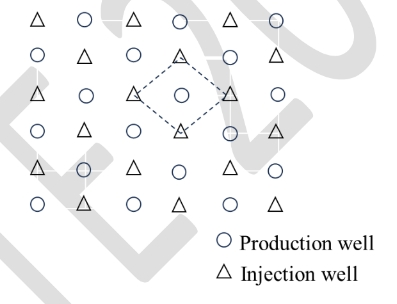
\includegraphics[width=0.5\columnwidth]{figs/im 6.jpeg}
    \caption{}
    \label{fig:placeholder}
\end{figure}


\begin{enumerate}
\begin{multicols}{2}
    \item 2
    \item 1
    \item $\frac{1}{4}$
    \item $\frac{1}{2}$
    \end{multicols}
\end{enumerate}
\hfill{\brak{\text{GATE PE 2024}}}



\item  Which ONE of the following options represents the waves generated during partitioning of acoustic energy at an interface inside the Earth?
\begin{enumerate}
\begin{multicols}{2}
    \item Rayleigh waves
    \item Love waves
    \item Body waves
    \item Surface waves
    \end{multicols}
\end{enumerate}
\hfill{\brak{\text{GATE PE 2024}}}



\item  "Earth is a low-pass filter". This implies it filters out which ONE of the following parameters in the subsurface?
\begin{enumerate}
\begin{multicols}{2}
    \item Phase
    \item Amplitude
    \item Frequency
    \item Velocity
    \end{multicols}
\end{enumerate}
\hfill{\brak{\text{GATE PE 2024}}}



 \item Which ONE is the correct formula for calculation of Foldage of a 2D seismic line?
\begin{enumerate}
    \item $\text{Foldage} = \left(\frac{1}{2}\right) \text{(number of geophones)} \left(\frac{\text{geophone interval spacing}}{\text{shot interval spacing}}\right)$
    \item $\text{Foldage} = \left(\frac{1}{2}\right) \text{(number of geophones)} \left(\frac{\text{shot interval spacing}}{\text{geophone interval spacing}}\right)$
    \item $\text{Foldage} = \left(\frac{1}{2}\right) \text{(number of shots)} \left(\frac{\text{shot interval spacing}}{\text{geophone interval spacing}}\right)$
    \item $\text{Foldage} = \left(\frac{1}{2}\right) \text{(number of shots)} \left(\frac{\text{geophone interval spacing}}{\text{shot interval spacing}}\right)$
\end{enumerate}
\hfill{\brak{\text{GATE PE 2024}}}



\item  Well tests can be classified as either 'single well productivity test' or 'descriptive reservoir test'. Which ONE of the following CANNOT be determined from a 'single well productivity test'?
\begin{enumerate}
    \item Characteristics of the formation damage and other source of skin
    \item Well deliverability
    \item Characteristics of both vertical and horizontal reservoir heterogeneity
    \item Identification of produced fluids and their respective volume ratios
\end{enumerate}
\hfill{\brak{\text{GATE PE 2024}}}



\item  Which mud type will have the highest acoustic velocity from the following options?
\begin{enumerate}
    \item Mud with live oil at low temperature
    \item Mud with dead oil at high temperature
    \item Mud with live oil at high temperature
    \item Mud with dead oil at low temperature
\end{enumerate}
\hfill{\brak{\text{GATE PE 2024}}}



 For the given matrix $Q = \myvec{ 
\frac{1}{\sqrt{2}} & 0 & \frac{1}{\sqrt{2}} \\ 
0 & 1 & 0 \\ 
-\frac{1}{\sqrt{2}} & 0 & \frac{1}{\sqrt{2}} 
}$, which of the following statements is/are true?
\begin{enumerate}
\begin{multicols}{2}
    \item $Q$ is an orthogonal matrix
    \item $Q^T = Q^{-1}$
    \item $Q$ is a singular matrix
    \item $Q$ is a symmetric matrix
    \end{multicols}
\end{enumerate}
\hfill{\brak{\text{GATE PE 2024}}}



\item  Which of the following is/are thermal enhanced oil recovery method(s)?
\begin{enumerate}
\begin{multicols}{2}
    \item Alkali-surfactant-polymer flooding
    \item In situ combustion
    \item Steam assisted gravity drainage
    \item Low salinity water flooding
    \end{multicols}
\end{enumerate}
\hfill{\brak{\text{GATE PE 2024}}}



\item Dilute sodium hydroxide is used in oilfield operations for enhanced oil recovery. For economic reasons, sodium hydroxide is delivered on site as anhydrous solid beads/cakes. This compound must be diluted on site by mixing water. Which of the following precautions must be followed during handling and preparation of dilute sodium hydroxide?
\begin{enumerate}
    \item Use of Personal Protective Equipment \brak{PPE} while handling and processing sodium hydroxide
    \item Adequate ventilation to avoid exposure of sodium hydroxide aerosols
    \item Stable supply of hot utility line as sodium hydroxide dilution is an endothermic reaction
    \item Stable supply of cold utility line as sodium hydroxide dilution is an exothermic reaction
\end{enumerate}
\hfill{\brak{\text{GATE PE 2024}}}
\item  If $P = \myvec{ 2 & -1 \\ 2 & 2 }$, the product of the eigenvalues of $P$ is \underline{\hspace{1cm}}.
\begin{enumerate}
\begin{multicols}{2}
    \item 2
    \item 4
    \item 6
    \item 8
    \end{multicols}
\end{enumerate}
\hfill{\brak{\text{GATE PE 2024}}}



\item  The number of ways in which a supervisor can choose four workers out of 10 equally competent workers is \underline{\hspace{1cm}}.
\begin{enumerate}
\begin{multicols}{2}
    \item 40
    \item 210
    \item 5040
    \item 10000
    \end{multicols}
\end{enumerate}
\hfill{\brak{\text{GATE PE 2024}}}



\item  A field rotational viscometer containing a drilling fluid gives a dial reading of $12^\circ$ and $20^\circ$ at rotor speeds of 300 rpm and 600 rpm, respectively. The drilling fluid is assumed to obey power law model, $\tau = K \dot{\gamma}^n$, where $\tau$ is the shear stress, $\dot{\gamma}$ is the shear rate, $K$ is the consistency index and $n$ is the power law index. The power law index, $n$, is \underline{\hspace{1cm}} \brak{\text{round off to two decimal places}}.
\begin{enumerate}
\begin{multicols}{4}
    \item 0.42
    \item 0.58
    \item 0.74
    \item 0.86
    \end{multicols}
\end{enumerate}
\hfill{\brak{\text{GATE PE 2024}}}



\item  Shear wave velocity \brak{\text{$V_s$}} in a limestone formation is 3600 m/s. Assume that the modulus of incompressibility \brak{\text{$K$}} is twice that of the modulus of rigidity \brak{\text{$G$}}, and the bulk density \brak{\text{$\rho_b$}} of the formation is 2700 kg/m$^3$. For this limestone formation, the compressional wave velocity \brak{\text{$V_p$}} is \underline{\hspace{1cm}} m/s.
\begin{enumerate}
\begin{multicols}{2}
    \item 4800
    \item 5400
    \item 6000
    \item 7200
   \end{multicols} 
\end{enumerate}
\hfill{\brak{\text{GATE PE 2024}}}



 \item Two reservoir sands A and B of same thickness are encountered in a well at different depths. The hydrocarbon in the shallow reservoir sand A is 10$^\circ$API whereas, in the deeper reservoir sand B, it is 20$^\circ$API. For single phase incompressible systems, it may be assumed that the permeability in the deeper reservoir sand B is half of that of the shallow reservoir sand A, and the viscosity is directly proportional to the specific gravity of oil in respective sands. The ratio of the mobility in reservoir sand A to that of reservoir sand B is \underline{\hspace{1cm}} \brak{\text{round off to two decimal places}}.
\begin{enumerate}
\begin{multicols}{2}
    \item 0.25
    \item 0.50
    \item 1.00
    \item 2.00
    \end{multicols}
\end{enumerate}
\hfill{\brak{\text{GATE PE 2024}}}
\item  Which ONE of the following is the implicit form of the solution for the differential equation given below?
\begin{align}
 \frac{dy}{dx} + \frac{2x+3y}{3x+5y} = 0  
\end{align}
Note: C in the options below is the integration constant.
\begin{enumerate}
\begin{multicols}{2}
    \item $x^2 - 3xy - \frac{5y^2}{2} - C = 0$
    \item $x^2 - 3xy + \frac{5y^2}{2} - C = 0$
    \item $x^2 + 3xy - \frac{5y^2}{2} - C = 0$
    \item $x^2 + 3xy + \frac{5y^2}{2} - C = 0$
    \end{multicols}
\end{enumerate}
\hfill{\brak{\text{GATE PE 2024}}}



\item $r(t) = \frac{\sin 3t}{t} \vec{i} + (t + 2)^4 \vec{j} + (t + 1)\frac{\sin t}{t} \vec{k}$, with $\vec{i}, \vec{j},$ and $\vec{k}$ being the unit vectors along $x, y$ and $z$ directions, respectively. The value of $\lim\limits_{t \to 0} r(t)$ is \underline{\hspace{1cm}}.
\begin{enumerate}
\begin{multicols}{2}
    \item 0
    \item $t + 32\vec{j} - \vec{k}$
    \item $3\vec{i} + 16\vec{j} + \vec{k}$
    \item $3\vec{i} + 16\vec{j}$
    \end{multicols}
\end{enumerate}
\hfill{\brak{\text{GATE PE 2024}}}



\item  From the following figure, match the CORRECT set of liquid shrinkage curves from GROUP I with various crude oil systems from GROUP II.
\begin{figure}[h]
    \centering
    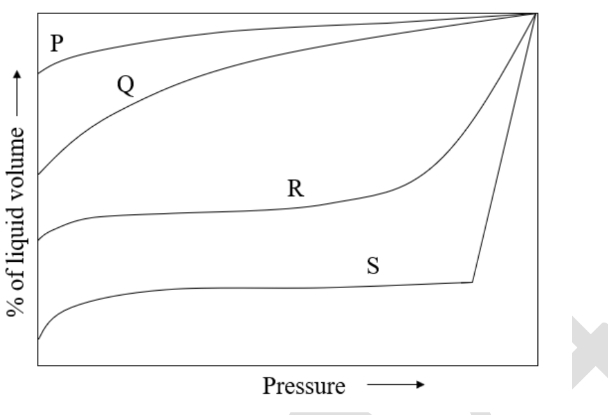
\includegraphics[width=0.5\columnwidth]{figs/im 7.jpeg}
    \caption{}
    \label{fig:placeholder}
\end{figure}


\begin{center}
[Figure showing curves P, Q, R, S]
\end{center}

\begin{table}[h!]
\centering
\[
\begin{array}{|l|l|}
\hline
\textbf{GROUP I} & \textbf{GROUP II} \\
\hline
(P)\ \text{Curve P} & (I)\ \text{High shrinkage crude oil} \\
(Q)\ \text{Curve Q} & (II)\ \text{Low shrinkage crude oil} \\
(R)\ \text{Curve R} & (III)\ \text{Ordinary black oil} \\
(S)\ \text{Curve S} & (IV)\ \text{Near-critical crude oil} \\
\hline
\end{array}
\]
\caption{Matching of crude oil types with PVT curves}
\label{tab:curves}
\end{table}


\begin{enumerate}
\begin{multicols}{2}
    \item P - I; Q - II; R - III; S - IV
    \item P - I; Q - III; R - IV; S - II
    \item P - II; Q - III; R - I; S - IV
    \item P - II; Q - IV; R - I; S - III
   \end{multicols} 
\end{enumerate}
\hfill{\brak{\text{GATE PE 2024}}}



\item  Match the following pressure-volume-temperature (PVT) studies from GROUP I with their objectives from GROUP II.

\begin{table}[h!]
\centering
\[
\begin{array}{|l|l|}
\hline
\textbf{GROUP I} & \textbf{GROUP II} \\
\hline
(P)\ \text{Constant composition expansion} & (I)\ \text{to determine the minimum miscibility pressure for gas injection} \\
(Q)\ \text{Differential liberation} & (II)\ \text{to determine the saturation pressure of the crude oil} \\
(R)\ \text{Separator test} & (III)\ \text{to mimic the reservoir performance during production} \\
(S)\ \text{Slim tube experiment} & (IV)\ \text{to design and optimize the separator conditions} \\
\hline
\end{array}
\]
\caption{Matching of PVT experiments with their applications}
\label{tab:pvt}
\end{table}
\begin{enumerate}
\begin{multicols}{2}
    \item P - III; Q - II; R - IV; S - I
    \item P - III; Q - IV; R - I; S - II
    \item P - II; Q - I; R - IV; S - III
    \item P - II; Q - III; R - IV; S - I
    \end{multicols}
\end{enumerate}
\hfill{\brak{\text{GATE PE 2024}}}
\item  Hydrocarbon fluids usually are classified as dry gas, wet gas, gas condensate and black oil. Which ONE of the following combinations is the CORRECT pressure - temperature phase diagram that represents the reservoir fluid type?
\begin{figure}[h]
    \centering
    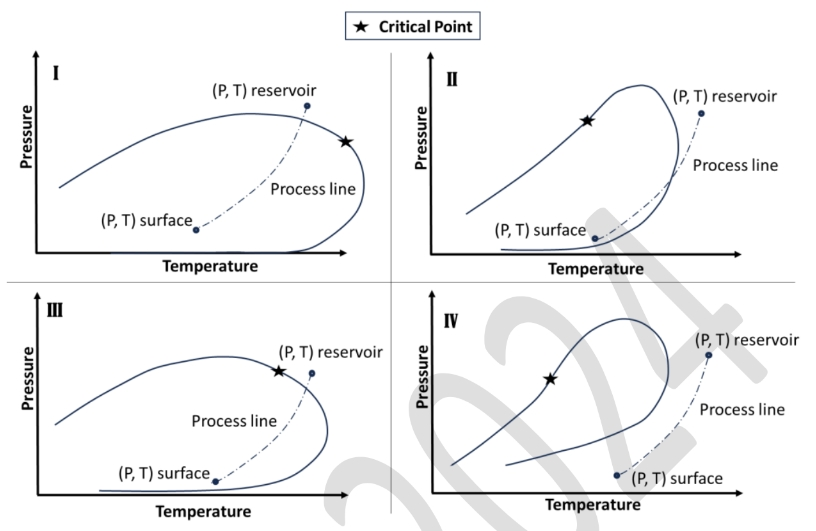
\includegraphics[width=0.5\columnwidth]{figs/im 8.jpeg}
    \caption{}
    \label{fig:placeholder}
\end{figure}
[Four phase diagrams labeled I, II, III, IV]

\begin{enumerate}
    \item I - dry gas; II - wet gas; III - gas condensate; IV - black oil
    \item I - dry gas; II - gas condensate; III - wet gas; IV - black oil
    \item I - black oil; II - wet gas; III - gas condensate; IV - dry gas
    \item I - gas condensate; II - black oil; III - wet gas; IV - dry gas
\end{enumerate}
\hfill{\brak{\text{GATE PE 2024}}}
\item  Which ONE of the following is the CORRECT combination?

\begin{table}[h!]
\centering
\[
\begin{array}{|l|l|}
\hline
\textbf{Dimensionless Number} & \textbf{Ratio of the forces} \\
\hline
(P)\ \text{Froude Number}     & (I)\ \text{Inertia/Gravity} \\
(Q)\ \text{Capillary Number}  & (II)\ \text{Buoyancy/Capillary} \\
(R)\ \text{Reynolds Number}   & (III)\ \text{Inertia/Viscous} \\
(S)\ \text{Bond Number}       & (IV)\ \text{Viscous/Capillary} \\
\hline
\end{array}
\]
\caption{Matching of dimensionless numbers with force ratios}
\label{tab:dimensionless}
\end{table}


\begin{enumerate}
\begin{multicols}{2}
    \item P - I; Q - IV; R - II; S - III
    \item P - II; Q - IV; R - III; S - I
    \item P - I; Q - IV; R - III; S - II
    \item P - I; Q - III; R - II; S - IV
    \end{multicols}
\end{enumerate}
\hfill{\brak{\text{GATE PE 2024}}}



 \item From the standard flexible riser configurations shown schematically in the figure, choose the CORRECT combination.
\begin{figure}[h]
    \centering
    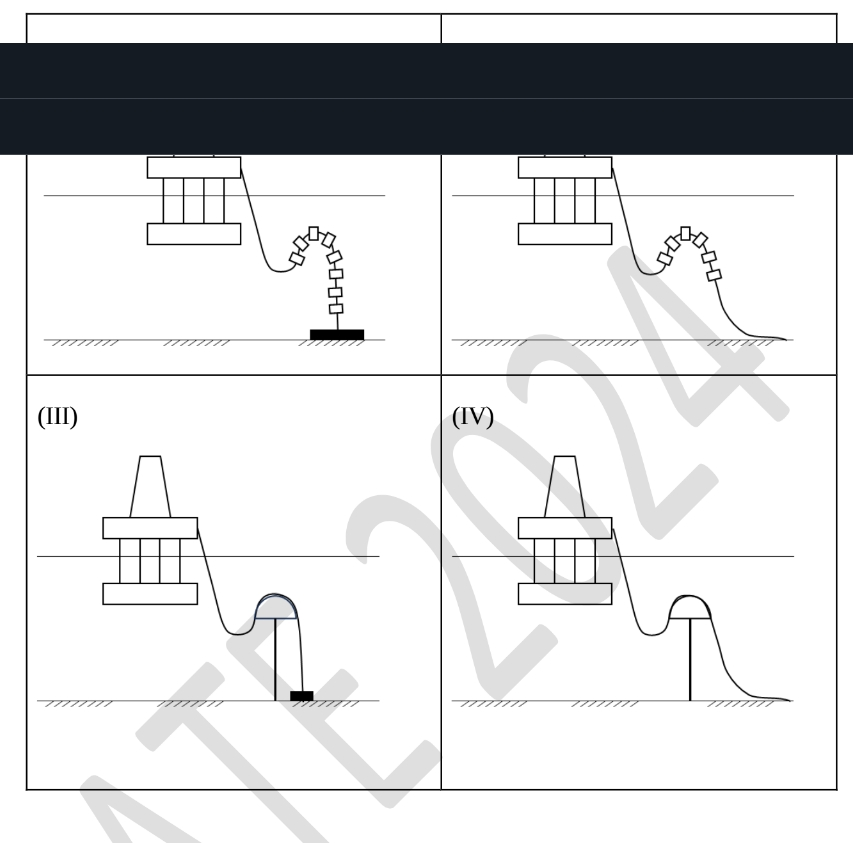
\includegraphics[width=0.5\columnwidth]{figs/im 9.jpeg}
    \caption{}
    \label{fig:placeholder}
\end{figure}
\begin{enumerate}
    \item I - Steep Wave; II - Lazy Wave; III - Steep S; IV - Lazy S
    \item I - Lazy Wave; II - Steep Wave; III - Lazy S; IV - Steep S
    \item I - Tethered Wave; II - Tethered S; III - Steep S; IV - Lazy S
    \item I - Steep Wave; II - Lazy Wave; III - Tethered S; IV - Tethered Wave
\end{enumerate}
\hfill{\brak{\text{GATE PE 2024}}}
\item  The figures below show the typical geometry of the subsurface strata in relation to the boundaries of the depositional sequences.
\begin{figure}[h]
    \centering
    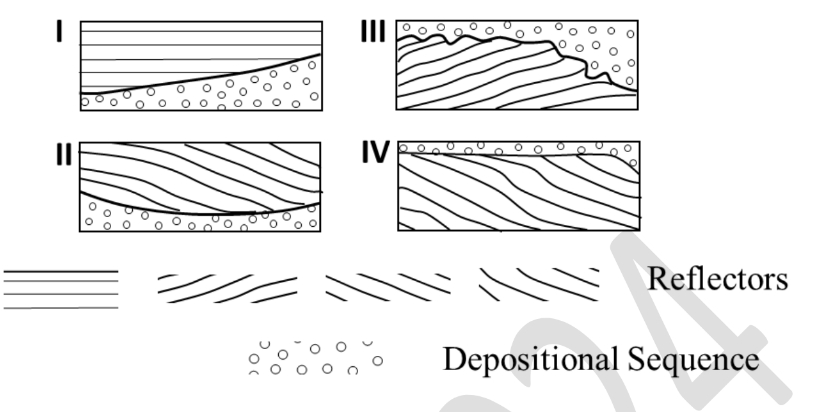
\includegraphics[width=0.5\columnwidth]{figs/im 10.jpeg}
    \caption{}
    \label{fig:placeholder}
\end{figure}
 Which ONE of the following options CORRECTLY represents the four seismic sequences with their corresponding names?

\begin{enumerate}
    \item I - Onlap; II - Toplap; III - Erosional truncation; IV - Downlap
    \item I - Onlap; II - Downlap; III - Erosional truncation; IV - Toplap
    \item I - Erosional truncation; II - Toplap; III - Onlap; IV - Downlap
    \item I - Erosional truncation; II - Downlap; III - Onlap; IV - Toplap
\end{enumerate}
\hfill{\brak{\text{GATE PE 2024}}}
\item  Which of the following tests is/are used to obtain reservoir deliverability \(\frac{kh}{\mu}\) information?
\begin{enumerate}[label=\arabic*.]
    \item Exploration or appraisal well openhole wireline
    \item Exploration or appraisal well Drill Stem Test (DST)
    \item Development well openhole wireline
    \item Development well Drill Stem Test (DST)
\end{enumerate}
\begin{enumerate}
\begin{multicols}{2}
    \item 1 only
    \item 3 only
    \item 1 and 3
    \item 2 and 4
    \end{multicols}
\end{enumerate}
\hfill{\brak{\text{GATE PE 2024}}}
\item  The decay of Gamma ray energy in the Earth formation goes through three dominant processes represented by regions I, II, and III in the figure below.
\begin{figure}[h]
    \centering
    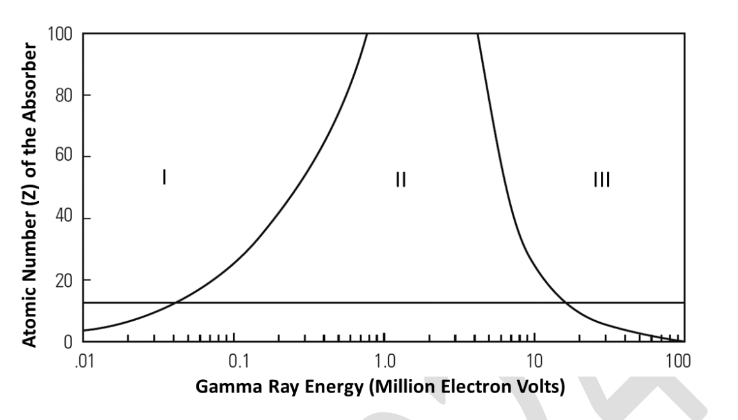
\includegraphics[width=0.5\columnwidth]{figs/im 11.jpeg}
    \caption{}
    \label{fig:placeholder}
\end{figure}
[Gamma ray energy decay diagram]

Which ONE of the following options is CORRECT?

\begin{enumerate}
    \item I - Photoelectric effect; II - Pair production effect; III - Compton effect
    \item I - Epithermal effect; II - Pair production effect; III - Photoelectric effect
    \item I - Photoelectric effect; II - Compton effect; III - Pair production effect
    \item I - Epithermal effect; II - Photoelectric effect; III - Compton effect
\end{enumerate}
\hfill{\brak{\text{GATE PE 2024}}}



 \item Consider single-phase radial flow of a fluid with constant viscosity and low compressibility through a homogenous and isotropic reservoir of constant porosity, permeability, and thickness. Match the flow regime with the CORRECT mathematical relation given in the table. P represents pressure, r represents the radial coordinate, and t represents time. f(r,t) is a function of 'r' and 't'.

\begin{table}[h!]
\centering
\[
\begin{array}{|l|l|}
\hline
\textbf{Flow regime} & \textbf{Mathematical relation} \\
\hline
(P)\ \text{Steady-state flow}        & (I)\ \left(\tfrac{\partial P}{\partial t}\right)_r = 0 \\
(Q)\ \text{Transient flow}           & (II)\ \left(\tfrac{\partial P}{\partial t}\right)_r = \text{constant} \\
(R)\ \text{Pseudosteady-state flow}  & (III)\ \left(\tfrac{\partial P}{\partial t}\right)_r = f(r,t) \\
\hline
\end{array}
\]
\caption{Matching of flow regimes with their mathematical relations}
\label{tab:flow}
\end{table}


\begin{enumerate}
\begin{multicols}{2}
    \item P - I; Q - II; R - III
    \item P - I; Q - III; R - II
    \item P - II; Q - III; R - I
    \item P - II; Q - I; R - III
    \end{multicols}
\end{enumerate}
\hfill{\brak{\text{GATE PE 2024}}}
 \item The microbial enhanced oil recovery method helps to recover oil by which one or more of the following phenomena?
\begin{enumerate}
    \item Reducing the interfacial tension due to production of biosurfactants
    \item Stimulating the well due to production of acids
    \item Increasing the mobility ratio due to production of biopolymers
    \item Reducing the viscosity due to production of gases in situ
\end{enumerate}
\hfill{\brak{\text{GATE PE 2024}}}




\item  Fixed roof tank for storage of organic liquids reduces volatile organic compound \brak{VOC} emissions and protects the stored liquid from elements and contamination. Such tanks are generally equipped with a vent at the roof. The objective\brak{s} of such a vent is/are to
\begin{enumerate}
    \item control pressure build-up in the tank
    \item control vacuum generation in the tank
    \item add oil to the tank
    \item add water to the tank
\end{enumerate}
\hfill{\brak{\text{GATE PE 2024}}}



\item  A choke is generally installed at the well head and/or downhole. The desired function\brak{s} of the choke is/are to
\begin{enumerate}
    \item protect surface equipment from damage
    \item avoid sand ingress problem
    \item regulate production rate
    \item ensure oil and water coning
\end{enumerate}
\hfill{\brak{\text{GATE PE 2024}}}



\item  Which of the following options is/are CORRECT about the below mentioned hydrocarbons? 
LNG: Liquefied Natural Gas; LPG: Liquefied Petroleum Gas; NGL: Natural Gas Liquid; CNG: Compressed Natural Gas
\begin{enumerate}
    \item LNG is primarily methane at approximately 110 K temperature
    \item LPG is primarily propane and butane at standard temperature and pressure
    \item NGL is primarily methane at standard temperature and pressure
    \item CNG is primarily pentane at standard temperature and pressure
\end{enumerate}
\hfill{\brak{\text{GATE PE 2024}}}




\item  Consider flow of two immiscible viscous fluids inside a thin slit of width $2B$. The flow rates of both the fluids are such that the planar interface is exactly at the center of the slit \brak{\text{corresponding to $X = 0$}}. The upper and lower fluid-solid boundaries lie at $X = B$ and $X = -B$, respectively. $\tau_{XZ}^I$ and $\tau_{XZ}^{II}$ are the shear stresses in fluids I and II, respectively. $v_Z^I$ and $v_Z^{II}$ are the velocities of fluid I and II, respectively in the $Z$ direction.

Which of the following options represent(s) the CORRECT boundary condition(s)?
\begin{figure}[h]
    \centering
    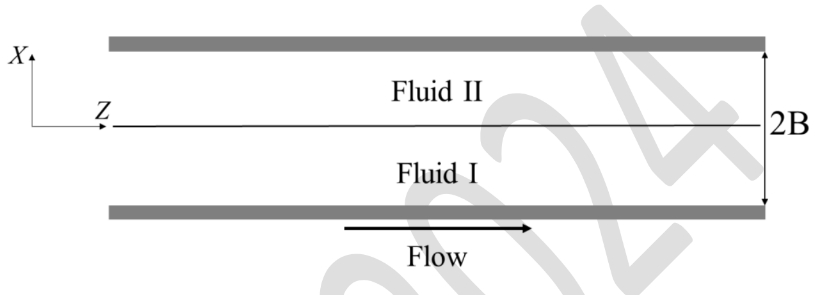
\includegraphics[width=0.5\columnwidth]{figs/im 12.jpeg}
    \caption{}
    \label{fig:placeholder}
\end{figure}

\begin{enumerate}
\begin{multicols}{2}
    \item At $X = 0$, $|\tau_{XZ}^I| = |\tau_{XZ}^{II}|$
    \item At $X = B$, $\tau_{XZ}^{II} = 0$
    \item At $X = B$, $v_Z^{II} = 0$
    \item At $X = -B$, $v_Z^I = 0$
    \end{multicols}
\end{enumerate}
\hfill{\brak{\text{GATE PE 2024}}}



\item  Given $f(x) = 2 + 20x + 30x^5$. The value of $\int_0^2 f(x) dx$ using Simpson's $\frac{1}{3}$rd rule with only one interior point is \underline{\hspace{1cm}}.
\begin{enumerate}
\begin{multicols}{2}
    \item 84
    \item 168
    \item 252
    \item 336
    \end{multicols}
\end{enumerate}
\hfill{\brak{\text{GATE PE 2024}}}



\item  If a weight of $P = 100$ N is supported by two massless strings connected to the walls as shown in the figure, the value of $T_1$ is \underline{\hspace{1cm}} N (round off to one decimal place).
\begin{figure}[h]
    \centering
    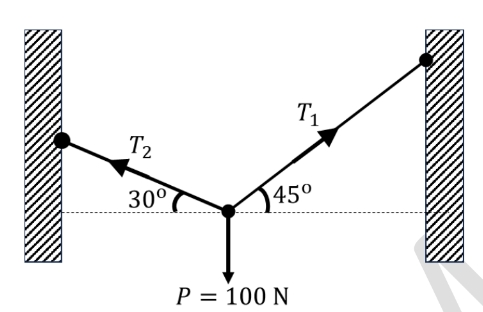
\includegraphics[width=0.5\columnwidth]{figs/im 13.jpeg}
    \caption{}
    \label{fig:placeholder}
\end{figure}

\begin{enumerate}
\begin{multicols}{4}
    \item 50.0
    \item 57.7
    \item 66.7
    \item 75.0
    \end{multicols}
\end{enumerate}
\hfill{\brak{\text{GATE PE 2024}}}



\item  Porosity and oil saturation of various core samples retrieved from a layered reservoir are given below. The thickness of different layers of the reservoir is also mentioned.

\begin{table}[h!]
\centering
\[
\begin{array}{|c|c|c|c|}
\hline
\textbf{Core sample} & \textbf{Layer thickness (ft)} & \textbf{Porosity (\%)} & \textbf{Oil saturation (\%)} \\
\hline
1 & 1.0 & 10 & 60 \\
2 & 1.5 & 15 & 65 \\
3 & 2.0 & 20 & 70 \\
4 & 2.5 & 25 & 75 \\
\hline
\end{array}
\]
\caption{Core sample properties}
\label{tab:core}
\end{table}


Assuming uniform area of cross section for all the layers, the average oil saturation of the reservoir is \underline{\hspace{1cm}} \% \brak{\text{round off to one decimal place}}.
\begin{enumerate}
\begin{multicols}{2}
    \item 65.5
    \item 67.5
    \item 69.5
    \item 71.5
    \end{multicols}
\end{enumerate}
\hfill{\brak{\text{GATE PE 2024}}}



 \item A natural gas has the following composition:

\begin{table}[h!]
\centering
\[
\begin{array}{|c|c|c|}
\hline
\textbf{Component (i)} & \textbf{Mole fraction ($y_i$)} & \textbf{Molecular weight ($M_i$)} \\
\hline
\text{CO}_2     & 0.02 & 44 \\
\text{CH}_4     & 0.93 & 16 \\
\text{C}_2\text{H}_6 & 0.03 & 30 \\
\text{C}_3\text{H}_8 & 0.02 & 44 \\
\hline
\end{array}
\]
\caption{Gas mixture composition}
\label{tab:composition}
\end{table}


Assume compressibility factor, $Z = 0.82$, the universal gas constant, $R = 10.73 \frac{\text{psia ft}^3}{\text{lb-mole }^\circ\text{R}}$. Density of the natural gas at 2000 psia and 150 $^\circ$F is \underline{\hspace{1cm}} lb/ft$^3$ \brak{\text{round off to two decimal places}}.
\begin{enumerate}
\begin{multicols}{4}
    \item 4.85
    \item 5.15
    \item 5.45
    \item 5.75
    \end{multicols}
\end{enumerate}
\hfill{\brak{\text{GATE PE 2024}}}



 \item A surfactant enhanced oil recovery process has been employed using a five-spot injection pattern on a sandstone reservoir. The reservoir has the following properties:

\begin{itemize}
\item Reservoir area, $A = 20$ acres
\item Reservoir thickness, $h = 25$ ft
\item Porosity of the reservoir, $\Phi = 0.20$
\item Residual oil saturation at termination of waterflood, $S_{orw} = 0.30$
\item Residual oil saturation left by surfactant flood, $S_{orc} = 0.10$
\item Oil formation volume factor, $B_o = 1.05$ reservoir bbl/STB
\item Volumetric sweep efficiency, $E_v = 1$
\item Initial oil saturation of the reservoir = 0.75
\end{itemize}

The ratio of oil displaced due to surfactant flood to the original oil in place at reservoir condition is \underline{\hspace{1cm}} \brak{\text{round off to two decimal places}}.
\brak{\text{Take: 1 acre = 43560 ft$^2$, 1 bbl = 5.615 ft$^3$}}.
\begin{enumerate}
\begin{multicols}{4}
    \item 0.15
    \item 0.25
    \item 0.35
    \item 0.45
\end{multicols}    
\end{enumerate}
\hfill{\brak{\text{GATE PE 2024}}}



 \item An ideal mixture of benzene and toluene is in equilibrium at a pressure of 750 mm Hg, and temperature of 90 $^\circ$C. The concentration of benzene in the vapour phase in mole fraction is \underline{\hspace{1cm}} \brak{\text{round off to two decimal places}}.

Following data is given:
\[
\log_{10} P_i^0 = A_i - \frac{B_i}{T + C_i}
\]
\[
A_b = 7, B_b = 1200, C_b = 210
\]
\[
A_t = 7, B_t = 1300, C_t = 210
\]
where $T$ is the temperature in $^\circ$C, $A_i$, $B_i$ and $C_i$ are Antoine constants for component $i$, and $P_i^0$ is the vapour pressure of pure component $i$. The subscripts b and t represent benzene and toluene, respectively.
\begin{enumerate}
\begin{multicols}{4}
    \item 0.45
    \item 0.55
    \item 0.65
    \item 0.75
 \end{multicols}   
\end{enumerate}
\hfill{\brak{\text{GATE PE 2024}}}



 \item The diameter and draft of a freely floating classical upright spar without moonpool is 30 m and 75 m, respectively. The added mass in heave mode is 1.8 times the mass of the spar. The critical damping of the spar in heave mode is \underline{\hspace{1cm}} $\times 10^6$ kg/s \brak{\text{round off to one decimal place}}. Take $\pi = 3.14$, density of seawater = 1025 kg/m$^3$, acceleration due to gravity = 10 m/s$^2$.
\begin{enumerate}
\begin{multicols}{4}
    \item 3.5
    \item 4.5
    \item 5.5
    \item 6.5
    \end{multicols}
\end{enumerate}
\hfill{\brak{\text{GATE PE 2024}}}



\item  A long vertical hollow steel pipe used as a column in an offshore structure follows Euler's column theory. The length, outer diameter and thickness of the pipe are 30 m, 0.50 m, and 0.03 m, respectively. The Euler buckling load \brak{\text{assuming no environmental loads}} of the pipe pinned at both the ends, is \underline{\hspace{1cm}} kN \brak{\text{round off to one decimal place}}. Take $\pi = 3.14$, Young's modulus of elasticity for steel = 210 GPa.
\begin{enumerate}
\begin{multicols}{2}
    \item 1250.5
    \item 1375.5
    \item 1500.5
    \item 1625.5
 \end{multicols}   
\end{enumerate}
\hfill{\brak{\text{GATE PE 2024}}}



\item  A core sample from a well-consolidated sand has a length of 10 cm, diameter of 4 cm, and a resistance ($r$) of 100 $\Omega$ at $T_2 = 200^\circ$F when completely saturated with brine. The resistivity $R_w(T_1)$ of brine is 0.5 $\Omega$.m at $T_1 = 75^\circ$F. The cementation factor, $m = 2$ and the tortuosity factor, $a = 1$. Use $R_w(T_2) = R_w(T_1) \frac{T_1 + 6.77}{T_2 + 6.77}$ where $T_1$ and $T_2$ are in $^\circ$F. The porosity (in fraction) of the core sample using generalized Humble's formula at $200^\circ$F is \underline{\hspace{1cm}} \brak{text{round off to two decimal places}}.
\begin{enumerate}
\begin{multicols}{4}
    \item 0.15
    \item 0.20
    \item 0.25
    \item 0.30
\end{multicols}    
\end{enumerate}
\hfill{\brak{\text{GATE PE 2024}}}



 \item In an exploratory well, both clean and dirty reservoir sand with quartz as major mineralogy is encountered. The clean reservoir sand is completely devoid of shale. The fraction of shale volume \brak{\text{$V_{sh}$}} in the dirty reservoir sand is 25\% with grain density \brak{\text{$\rho_{sh}$}} of 2.7 g/cc. Quartz \brak{\text{$V_q$}} with grain density \brak{\text{$\rho_q$}} of 2.65 g/cc. The bulk density \brak{\text{$\rho_b$}} of the clean and the dirty reservoir sand is 2 g/cc and 2.25 g/cc, respectively, and the pore fluid density \brak{\text{$\rho_f$}} is 1 g/cc for both the sands. The difference of porosity \brak{\text{$\phi_{\text{clean}} - \phi_{\text{Dirty}}$}} in fraction between the two reservoir sands is \underline{\hspace{1cm}} \brak{\text{round off three decimal places}}.
\begin{enumerate}
\begin{multicols}{4}
    \item 0.075
    \item 0.100
    \item 0.125
    \item 0.150
 \end{multicols}   
\end{enumerate}
\hfill{\brak{\text{GATE PE 2024}}}



\item  The settling velocity \brak{\text{$v_s$}} of a spherical particle in a Newtonian fluid using Stokes' law is
\begin{align}
   v_s = \frac{g d_s^2 (\rho_s - \rho_l)}{18 \mu} 
\end{align}


where $d_s$ is the particle diameter, $\rho_s$ is the particle density, $\rho_l$ is the drilling fluid density, $\mu$ is the drilling fluid viscosity, and $g$ is acceleration due to gravity.

The density of barite and a drilled solid particle are 4200 kg/m$^3$ and 2600 kg/m$^3$, respectively. The density of the drilling fluid is 1300 kg/m$^3$. The diameter of a drilled spherical solid particle that has the same settling velocity as a spherical barite particle of 0.1 mm diameter in the drilling fluid is \underline{\hspace{1cm}} mm \brak{\text{round off to two decimal places}}.
\begin{enumerate}
\begin{multicols}{4}
    \item 0.12
    \item 0.14
    \item 0.16
    \item 0.18
  \end{multicols}  
\end{enumerate}
\hfill{\brak{\text{GATE PE 2024}}}



\item  A two-cylinder reciprocating positive-displacement mud pump is used for mud circulation. The pump can deliver fluid on both forward and backward piston strokes. The pump has the following specifications:
\begin{itemize}
\item Liner diameter = 15 cm
\item Piston rod diameter = 6 cm
\item Stroke length = 40 cm
\item Volumetric efficiency = 85\%
\end{itemize}
Take $\pi = 3.14$. The total volume of fluid displaced per complete pump cycle is \underline{\hspace{1cm}} cm$^3$.
\begin{enumerate}
\begin{multicols}{2}
    \item 10000
    \item 12000
    \item 14000
    \item 16000
\end{multicols}    
\end{enumerate}
\hfill{\brak{\text{GATE PE 2024}}}



\item  Consider the displacement of oil by water through a one-dimensional homogeneous isotropic porous medium of uniform porosity, permeability and thickness. Assume oil and water to be incompressible and immiscible. The relative permeabilities of oil \brak{\text{$k_{ro}$}} and water \brak{\text{$k_{rw}$}} at a given water saturation \brak{\text{$S_w$}} are:
\begin{align}
 k_{ro} = k_{ro}^0 (1 - S_w^*)\\
 k_{rw} = k_{rw}^0 S_w^*\\
 S_w^* = \frac{S_w - S_{wr}}{1 - S_{or} - S_{wr}}
\end{align}
where $k_{ro}^0$ and $k_{rw}^0$ are the end point relative permeabilities of oil and water, respectively. $S_{or}$ and $S_{wr}$ are the residual saturations of oil and water, respectively. Assume that $k_{ro}^0 = 0.8$, $k_{rw}^0 = 0.3$, $S_{or} = 0.35$, and $S_{wr} = 0.25$. The viscosities of water and oil are 1 cP and 8 cP, respectively. The mobility ratio corresponding to the water saturation ($S_w$) of 0.6 is \underline{\hspace{1cm}} (round off to one decimal place).
\begin{enumerate}
\begin{multicols}{2}
    \item 0.5
    \item 1.0
    \item 1.5
    \item 2.0
  \end{multicols}  
\end{enumerate}
\hfill{\brak{\text{GATE PE 2024}}}



\item  The invasion of a drilling fluid to a radius of 3 feet from the center of the well-bore into the formation has resulted in the development of skin. The permeability of the skin zone \brak{\text{region affected by the drilling fluid invasion}} is 50 mD. The permeability of the unaffected formation is 400 mD. The well bore radius is 0.25 feet. The value of the skin factor is \underline{\hspace{1cm}} \brak{\text{round off to two decimal places}}.
\begin{enumerate}
\begin{multicols}{2}
    \item 2.08
    \item 3.08
    \item 4.08
    \item 5.08
    \end{multicols}
\end{enumerate}
\hfill{\brak{\text{GATE PE 2024}}}

\begin{center}
\textbf{\large --- END OF THE QUESTION PAPER---}
\end{center}
\end{enumerate}
\end{document}